\documentclass[11pt]{scrartcl}
\usepackage{polski}
\usepackage[polish]{babel}

\usepackage{graphicx, float, caption, subcaption, amsmath}
\usepackage{tabularx, multirow, hyperref, enumitem, listings}
\usepackage{xcolor}
%\usepackage{minted}

\hypersetup{
    colorlinks=true,
    linkcolor=black,
    urlcolor=black,
    citecolor=black
}

\definecolor{md-black}{rgb}{0.12, 0.12, 0.12}
\definecolor{md-teal}{rgb}{0.38, 0.79, 0.69}
\definecolor{md-mauve}{rgb}{0.76, 0.52, 0.75}
\definecolor{md-green}{rgb}{0.13, 0.55, 0.13}
\definecolor{md-red}{rgb}{0.82, 0.10, 0.14}
\definecolor{md-purple}{rgb}{0.69, 0.33, 0.73}
\definecolor{md-orange}{rgb}{0.96, 0.42, 0.18}
\definecolor{md-gray}{rgb}{0.44, 0.46, 0.51}

\lstset{
    language=Python,
    basicstyle=\color{md-teal}\ttfamily,
    keywordstyle=\color{md-mauve},
    commentstyle=\color{md-green},
    stringstyle=\color{md-red},
    numbers=left,
    numberstyle=\small\color{md-gray}\ttfamily,
    stepnumber=1,
    numbersep=5pt,
    backgroundcolor=\color{md-black},
    showspaces=false,
    showstringspaces=false,
    showtabs=false,
    frame=none,
    tabsize=4,
    captionpos=b,
    breaklines=true,
    breakatwhitespace=false,
    escapeinside={\%*}{*)},
    numbersep=-10pt,
    morekeywords={as}
}

\graphicspath{{../images/}}

\title{Laboratorium 4 - Efekt Rungego}
\author{Mateusz Podmokły - II rok Informatyka WI}
\date{21 marzec 2024}

\begin{document}
    \maketitle

    \section{Treść zadania}
    \textbf{Zadanie 1.} Wyznacz wielomiany interpolujące funkcje:
    \[
        f_1(x)=\frac{1}{1+25x^2}, x \in [-1,1],
    \]
    \[
        f_2(x)=e^{cos(x)}, x \in [0,2\pi],
    \]
    używając:
    \begin{itemize}[label=--]
        \item wielomianów Lagrange'a z węzłami $x_j=x_0+jh, j=0,1,
            \ldots ,n, h=\frac{x_n-x_0}{n}$
        \item kubicznych funkcji sklejancyh z węzłami $x_j=x_0+jh,
            j=0,1, \ldots ,n, h=\frac{x_n-x_0}{n}$
        \item wielomianów Lagrange'a z węzłami Czebyszewa
        \[
            x_j=cos(\theta_j)
        \]
        \[
            \theta_j=\frac{2j+1}{2(n+1)}\pi, 0 \leq j \leq n.
        \]
    \end{itemize}
    Dla funkcji Rungego $f_1(x)$ wykonaj interpolację podanymi
    sposobami z $n=12$ węzłami interpolacji. Przedstaw na wykresie
    funkcję $f_1(x)$ oraz wyniki interpolacji. \\
    Wykonaj interpolację funkcji $f_1(x)$ i $f_2(x)$ podanymi
    sposobami z $n=4,5, \ldots ,50$ węzłami interpolacji. Przeprowadź
    ewaluację wyników na zbiorze 500 losowo wybranych punktów.
    Na wykresie przedstaw normę wektora błędu na tym zbiorze
    punktów w zależności od liczby węzłów interpolacji dla każdej
    metody, osobno dla obudwu funkcji.

    \section{Specyfikacja użytego środowiska}
    Specyfikacja:

    \begin{itemize}
        \item Środowisko: Visual Studio Code,
        \item Język programowania: Python,
        \item System operacyjny: Microsoft Windows 11,
        \item Architektura systemu: x64.
    \end{itemize}

    \section{Rozwiązanie problemu}
    W realizacji rozwiązania wykorzystane zostały następujące
    biblioteki:
    \begin{lstlisting}
        import numpy as np
        import matplotlib.pyplot as plt
    \end{lstlisting}

    \subsection*{}
    Obliczamy wielomian interpolacyjny Lagrange'a ze wzoru
    \[
        w(x)=\sum_{i=0}^{n}y_i \cdot \prod_{j=0 \land j \neq i}^{n}
        \frac{x-x_j}{x_i-x_j}
    \]
    Funkcje sklejane (splajny) obliczamy na każdym przedziale
    oddzielnie wykorzystując wielomiany Lagrange'a. Węzły
    Czebyszewa na przedziale $[-1,1]$ obliczamy ze wzoru
    \[
        x_j=cos(\theta_j)
    \]
    \[
        \theta_j=\frac{2j+1}{2(n+1)}\pi, 0 \leq j \leq n.
    \]
    Transformacja węzłów Czebyszewa $r \in [-1,1]$ na punkty
    $x \in [a,b]$ dana jest wzorem
    \[
        x=a+ \frac{(b-a)(r+1)}{2}
    \]
    Punkty do ewaluacji wylosowane zostały z użyciem funkcji
    \texttt{np.random.uniform}, następnie obliczona została norma
    wektora błędu względnego interpolacji za pomocą funkcji
    \texttt{np.linalg.norm}.
    
    \section{Przedstawienie wyników}

    \subsection{Interpolacja funkcji Rungego}
    \begin{figure}[H]
        \centering
        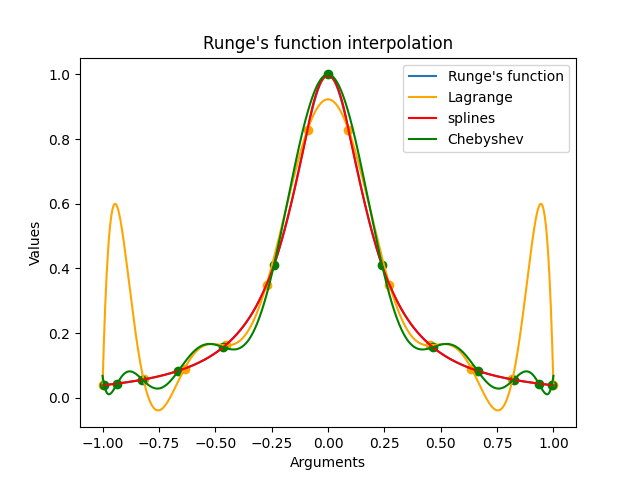
\includegraphics[width=0.8\linewidth]{interpolation1.png}
        \caption{Porównanie uzyskanych interpolacji.}
    \end{figure}

    \subsection{Porównanie dokładności różnych metod interpolacji}
    \begin{figure}[H]
        \centering
        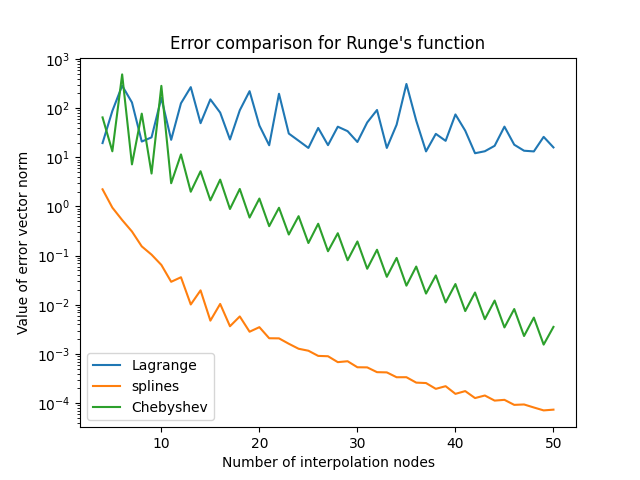
\includegraphics[width=0.75\linewidth]{interpolation2.png}
        \caption{Wykres błędów interpolacji funkcji Rungego.}
    \end{figure}
    \begin{figure}[H]
        \centering
        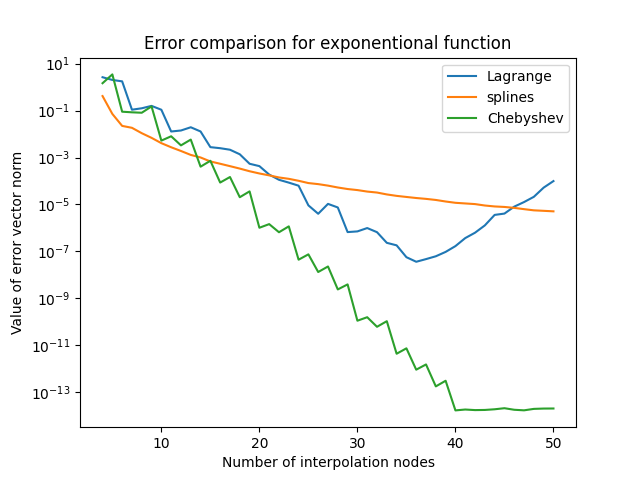
\includegraphics[width=0.75\linewidth]{interpolation3.png}
        \caption{Wykres błędów interpolacji funkcji eksponencjalnej.}
    \end{figure}

    W przypadku funkcji Rungego, najbardziej dokładna jest
    interpolacja funkcjami sklejanymi (splajnami). Funkcję
    eksponencjalną najlepiej interpoluje wielomian Lagrange'a
    z węzłąmi Czebyszewa. Przy zwiększaniu liczby węzłów interpolacji
    rośnie dokładność, jedynie dla funkcji eksponencjalnej
    interpolowanej wielomianem Lagrange'a od około 40 węzłów
    dokładność zaczyna maleć.

    \section{Wnioski}
    \subsection{Obserwacje}
    Interpolacja funkcji Rungego wielomianem Lagrange'a z równoodległymi
    węzłami powoduje duże niedokładności, szczególnie na krańcach
    przedziału. Wykorzystanie węzłów Czebyszewa znacznie zmniejsza ten
    efekt, natomiast najwyższą dokładność gwarantuje użycie do tego celu
    funkcji sklejanych (splajnów). Może to wynikać z faktu, że dla
    każdego przedziału dobieramy inny wielomian interpolacyjny, co
    pozwala lepiej dopasować interpolację do funkcji. \\
    Dla funkcji eksponencjalnej natomiast, dokładniejsza okazała
    się interpolacja Lagrange'a z wykorzystaniem węzłów Czebyszewa,
    które pozwalają w lepszy sposób dobrać węzły interpolacji i dzięki
    temu uniknąć dużych niedokładności. \\
    Wyższa dokładność przy większej liczbie węzłów interpolacji
    jest spowodowana lepiej dopasowanym wielomianem interpolacyjnym
    do danej funkcji, jedynym wyjątkiem tutaj jest interpolacja
    Lagrane'a funkcji eksponencjalnej.

    \subsection{Podsumowanie}
    W przypadku niektórych funkcji zwykła interpolacja wielomianem
    Lagrange'a okazuje się bardzo niedokładna, szczególnie na
    krańcach przedziału. Należy wtedy zastosować inne techniki
    interpolacji, jak na przykład węzły Czebyszewa, albo funkcje
    sklejane, tzw. splajny. Pozwala to w takich sytuacjach zachować
    wyższą dokładność.

    \section{Bibliografia}
    \url{https://pl.wikipedia.org/wiki/Funkcja_wyk%C5%82adnicza} \\
    \url{https://pl.wikipedia.org/wiki/W%C4%99z%C5%82y_Czebyszewa} \\
    \url{https://pl.wikipedia.org/wiki/Funkcja_sklejana} \\
    \url{https://pl.wikipedia.org/wiki/Interpolacja_funkcjami_
        sklejanymi}

\end{document}
